\documentclass[10pt,a4paper]{article}

% ===============================================================================
% PREAMBLE & PACKAGES
% ===============================================================================
\usepackage{fontspec}
\setmainfont{Latin Modern Roman}
\setmonofont{Latin Modern Mono}
\usepackage{unicode-math}
\setmathfont{Latin Modern Math}

\usepackage[margin=0.7in,top=0.9in,bottom=0.9in]{geometry}
\usepackage{xcolor}
\usepackage{tikz}
\usetikzlibrary{shapes.geometric, arrows.meta, positioning, calc, fit, decorations.pathreplacing}
\usepackage[most]{tcolorbox}
\usepackage{tabularx}
\usepackage{array}
\usepackage{enumitem}
\usepackage{amsmath}
\usepackage{fancyhdr}
\usepackage{microtype}
\usepackage[colorlinks=true,linkcolor=myteal,citecolor=mypurple,urlcolor=myblue]{hyperref}

\hyphenpenalty=10000
\exhyphenpenalty=10000
\sloppy

% ===============================================================================
% COLOR PALETTE (Strict adherence to spec)
% ===============================================================================
\definecolor{myred}{RGB}{196,30,58}       % section headings
\definecolor{mydark}{RGB}{30,30,50}       % body text
\definecolor{mygreen}{RGB}{14,120,80}     % definition boxes
\definecolor{myteal}{RGB}{0,130,140}      % formula boxes, diagrams, subsection headings
\definecolor{myamber}{RGB}{180,100,0}     % example boxes
\definecolor{mypurple}{RGB}{100,30,160}   % exam/viva boxes
\definecolor{myblue}{RGB}{25,90,170}      % hyperlinks/diagrams
\definecolor{mygray}{RGB}{246,247,249}    % tikzbox background
\definecolor{mgframe}{RGB}{180,185,200}   % tikzbox border
\definecolor{watermark}{RGB}{145,150,170} % footer watermark

\definecolor{hdrred}{RGB}{250,232,235}
\definecolor{hdrgreen}{RGB}{220,244,233}
\definecolor{hdrteal}{RGB}{220,242,244}
\definecolor{hdramber}{RGB}{253,242,215}
\definecolor{hdrpurple}{RGB}{238,228,255}
\definecolor{hdrblue}{RGB}{235,242,250}

% ===============================================================================
% TCOLORBOX STYLES
% ===============================================================================
\tcbset{
  tikzbox/.style={colback=mygray, colframe=mgframe, boxrule=0.6pt, arc=4pt,
    left=8pt, right=8pt, top=6pt, bottom=6pt,
    colbacktitle=mgframe, coltitle=mydark, fonttitle=\small\bfseries},
  defbox/.style={colback=hdrgreen, colframe=mygreen, boxrule=0.8pt, arc=4pt,
    left=9pt, right=9pt, top=6pt, bottom=6pt,
    colbacktitle=mygreen, coltitle=white, fonttitle=\small\bfseries},
  formulabox/.style={colback=hdrteal, colframe=myteal, boxrule=0.8pt, arc=4pt,
    left=9pt, right=9pt, top=7pt, bottom=7pt,
    colbacktitle=myteal, coltitle=white, fonttitle=\small\bfseries},
  examplebox/.style={colback=hdramber, colframe=myamber, boxrule=0.8pt, arc=4pt,
    left=9pt, right=9pt, top=6pt, bottom=6pt,
    colbacktitle=myamber, coltitle=white, fonttitle=\small\bfseries},
  masonbox/.style={colback=hdrpurple, colframe=mypurple, boxrule=0.8pt, arc=4pt,
    left=9pt, right=9pt, top=6pt, bottom=6pt,
    colbacktitle=mypurple, coltitle=white, fonttitle=\small\bfseries},
  exambox/.style={colback=hdrpurple, colframe=mypurple, boxrule=1pt, arc=5pt,
    left=10pt, right=10pt, top=8pt, bottom=8pt,
    colbacktitle=mypurple, coltitle=white, fonttitle=\bfseries,
    title after break={\textbf{Frequently Asked / Viva Questions (contd.)}}}
}
\tcbset{breakable}

% ===============================================================================
% TIKZ STYLES
% ===============================================================================
\tikzset{
  block/.style={rectangle, draw=myteal, fill=hdrteal, text width=2.4cm, align=center, minimum height=0.95cm, font=\small, rounded corners=3pt, line width=0.7pt},
  redblock/.style={rectangle, draw=myred, fill=hdrred, text width=2.4cm, align=center, minimum height=0.95cm, font=\small, rounded corners=3pt, line width=0.7pt},
  arrow/.style={-Stealth, thick, color=mydark},
  line/.style={thick, color=mydark}
}

% ===============================================================================
% MACROS & COMMANDS
% ===============================================================================
\newcommand{\Q}[1]{\textbf{#1}\par\vspace{2pt}}
\newcolumntype{Y}{>{\raggedright\arraybackslash}X}
\newcolumntype{C}{>{\centering\arraybackslash}X}

% Header & Footer
\pagestyle{fancy}
\fancyhf{}
\fancyhead[L]{\small\color{mydark}\textbf{OE-EC804B} --- Microwave Integrated Circuits}
\fancyhead[R]{\small\color{myteal}\textbf{Module 1 Notes}}
\fancyfoot[C]{\small\color{mydark}\thepage}
\fancyfoot[R]{\small\color{watermark}\copyright\ Biraj Sarkar}
\renewcommand{\headrulewidth}{0.6pt}

\hypersetup{pdftitle={OE-EC804B Module 1 Exam Notes}}

\begin{document}

% ===============================================================================
% TITLE BLOCK
% ===============================================================================
\begin{center}
  {\LARGE\bfseries\color{myred} OE-EC804B --- Microwave Integrated Circuits}\\[5pt]
  {\normalsize\color{mydark} Semester VIII \quad$\bullet$\quad 3L:0T:0P \quad$\bullet$\quad 3 Credits}\\[3pt]
  {\normalsize\color{myteal}\textbf{Module 1 Exam Notes: Introduction to MIC \& MMIC}}\\[3pt]
  {\small\color{mydark} CGEC \;$|$\; B.Tech ECE (2023--27) \;$|$\; \textit{Biraj Sarkar}}
\end{center}
\vspace{2pt}
\noindent{\color{myred}\rule{\linewidth}{1.5pt}}
\vspace{2pt}

\hypersetup{linkcolor=mydark}
\tableofcontents
\hypersetup{linkcolor=myteal}
\newpage

% ===============================================================================
% 1. INTRODUCTION TO MIC AND MMIC
% ===============================================================================
\section{Introduction to MIC and MMIC}

Microwave Integrated Circuits (MICs) operate in the high-frequency spectrum ranging from $300\text{ MHz}$ to $300\text{ GHz}$ (wavelengths $\lambda = 1\text{ m}$ to $1\text{ mm}$). Conventional low-frequency lumped elements (discrete resistors, capacitors, and inductors) fail at microwave frequencies due to parasitic lead inductances and stray capacitances. MIC technology replaces bulky 3D waveguide structures with planar transmission lines printed directly on insulating or semiconductor substrates.

\begin{tcolorbox}[defbox, title={Microwave Integrated Circuit (MIC)}]
  A \textbf{Microwave Integrated Circuit (MIC)} is a high-frequency planar assembly where passive circuit elements (printed microstrip lines, inductors, capacitors, couplers) and active semiconductor devices (diodes, MESFETs, HEMTs, HBTs) are integrated on a common planar substrate.
\end{tcolorbox}

\subsection{Classification: Hybrid MIC (HMIC) vs. Monolithic MIC (MMIC)}

MICs are categorized into two major technological generations:

\begin{enumerate}[leftmargin=*, itemsep=5pt]
  \item \textbf{Hybrid MIC (HMIC):} Passive matching networks and transmission lines are fabricated on a passive dielectric substrate (such as Alumina $\text{Al}_2\text{O}_3$, Quartz, or Sapphire) using thin or thick film deposition. Active semiconductor devices (packaged or unpackaged GaAs/Si FET dies, Schottky/PIN diodes) are individually mounted onto the substrate and connected using gold wire bonds or ribbon bonds.
  \item \textbf{Monolithic MIC (MMIC):} All active semiconductor devices (MESFETs, HEMTs, HBTs), passive matching components (MIM capacitors, thin film resistors, spiral inductors), and planar interconnect transmission lines are grown, etched, and metallized \textbf{simultaneously on a single semiconductor wafer} (such as Gallium Arsenide GaAs, Indium Phosphide InP, or Gallium Nitride GaN).
\end{enumerate}

\par\vspace{6pt}\noindent
\begingroup
\renewcommand{\arraystretch}{1.4}%
\begin{tabularx}{\linewidth}{|>{\raggedright\arraybackslash\bfseries}p{3.2cm}|Y|Y|}
\hline
\textbf{Feature} & \textbf{Hybrid MIC (HMIC)} & \textbf{Monolithic MIC (MMIC)} \\
\hline
Substrate Material & Dielectric (Alumina $\text{Al}_2\text{O}_3$, Quartz, Sapphire, PTFE) & Semi-insulating Semiconductor (GaAs, InP, GaN, SiGe) \\
\hline
Active Device Integration & Discrete semiconductor dies mounted \& wire-bonded individually & Fabricated monolithically directly inside/on the semiconductor wafer \\
\hline
Parasitic Reactance & High due to wire bond inductances ($L_s \approx 0.5 - 2\text{ nH}$) & Negligible; planar interconnects eliminate bond wire inductances \\
\hline
Frequency Range & Typically $< 20\text{ GHz}$ due to bond wire parasitics & Millimeter-wave up to $300\text{ GHz}$ and THz frequencies \\
\hline
Production Volume & Ideal for prototype development and low-volume production & Highly economical for mass batch production ($10^4 - 10^7$ units) \\
\hline
Unit Cost & Low initial mask cost; high unit assembly labor cost & High initial mask/NRE cost; extremely low per-chip unit cost \\
\hline
Post-Fabrication Tuning & Trimming of capacitors/resistors possible post-fabrication & No post-fabrication tuning possible; design must be 100\% accurate \\
\hline
Thermal Dissipation & Excellent thermal transfer through thick ceramic substrates & Moderate to poor; requires thermal via holes through wafer \\
\hline
\end{tabularx}
\endgroup

\subsection{Advantages of MICs over Discrete \& Waveguide Circuits}
\begin{itemize}[leftmargin=*, itemsep=4pt]
  \item \textbf{Miniaturization \& Weight Reduction:} Planar integration reduces volume and weight by over $90\%$ compared to metallic waveguides.
  \item \textbf{High Reliability \& Reproducibility:} Batch photolithography eliminates mechanical assembly variations and hand-soldered joints.
  \item \textbf{Broadband Performance:} Short planar interconnects minimize parasitic leads, extending operating bandwidths to multi-octave ranges.
  \item \textbf{Multifunctional Systems-on-Chip (SoC):} Enables complete transmit/receive (T/R) radar modules on a single die.
\end{itemize}

% ===============================================================================
% 2. MMIC FABRICATION TECHNIQUES AND MATERIALS
% ===============================================================================
\section{MMIC Fabrication Techniques and Materials}

\subsection{Substrate Materials for MMICs}
The choice of substrate dictates electrical attenuation, substrate power loss, high-frequency cutoff, and power dissipation capabilities.

\begin{tcolorbox}[masonbox, title={Substrate Requirements for MMICs}]
  An ideal MMIC substrate must exhibit:
  \begin{enumerate}[leftmargin=*, noitemsep]
    \item High electrical resistivity ($\rho > 10^7\text{ }\Omega\cdot\text{cm}$) to minimize RF substrate conduction losses.
    \item Low dielectric loss tangent ($\tan\delta < 0.001$) for minimal wave attenuation.
    \item High thermal conductivity ($K$) to dissipate heat from high-power active devices.
    \item High electron mobility ($\mu_e$) to enable high-speed transistor switching.
  \end{enumerate}
\end{tcolorbox}

\par\vspace{6pt}\noindent
\begingroup
\renewcommand{\arraystretch}{1.4}%
\begin{tabularx}{\linewidth}{|>{\raggedright\arraybackslash\bfseries}p{2.5cm}|>{\centering\arraybackslash}X|>{\centering\arraybackslash}X|>{\centering\arraybackslash}X|>{\raggedright\arraybackslash}X|}
\hline
\textbf{Substrate} & \textbf{Dielectric Constant ($\varepsilon_r$)} & \textbf{Loss Tangent ($\tan\delta$)} & \textbf{Thermal Cond. ($W/cm\cdot K$)} & \textbf{Key Properties \& Applications} \\
\hline
Gallium Arsenide (GaAs) & $12.9$ & $0.0006$ & $0.46$ & Standard workhorse for MMICs up to $100\text{ GHz}$; high mobility ($\mu_e = 8500\text{ cm}^2/\text{V}\cdot\text{s}$). \\
\hline
Indium Phosphide (InP) & $12.4$ & $0.0010$ & $0.68$ & Sub-millimeter wave and THz MMICs ($>100\text{ GHz}$); ultra-high peak electron velocity. \\
\hline
Gallium Nitride (GaN) & $8.9$ & $0.0005$ & $1.30$ & High-power microwave amplifiers; high breakdown field ($3\text{ MV/cm}$). \\
\hline
Silicon (Si / High-Res) & $11.7$ & $0.0050$ & $1.45$ & RF-CMOS and SiGe HBT integration; cheap mass production up to $60\text{ GHz}$. \\
\hline
Alumina ($\text{Al}_2\text{O}_3$) & $9.8$ & $0.0001$ & $0.30$ & Standard substrate for Hybrid MICs; excellent dielectric stability. \\
\hline
\end{tabularx}
\endgroup

\subsection{Thin Film Technology (Film Thickness \texorpdfstring{$< 5\text{ }\mu\text{m}$}{< 5 um})}
Thin film technology is used in all high-frequency MMICs and precision Hybrid MICs.

\begin{itemize}[leftmargin=*, itemsep=4pt]
  \item \textbf{Deposition Methods:}
    \begin{itemize}[leftmargin=*, noitemsep]
      \item \textit{Vacuum Evaporation:} Thermal or electron-beam heating vaporizes metal atoms in high vacuum ($10^{-6}\text{ Torr}$).
      \item \textit{RF Sputtering:} Argon ions bombard a target material, knocking off atoms that deposit uniformly onto the substrate.
      \item \textit{Electroplating:} Electro-chemical growth used to thicken conductor traces to several skin depths ($2-5\text{ }\mu\text{m}$ of Gold Au).
    \end{itemize}
  \item \textbf{Passive Component Fabrication:}
    \begin{itemize}[leftmargin=*, noitemsep]
      \item \textit{Thin Film Resistors:} Tantalum Nitride ($\text{TaN}$) or Nickel Chromium ($\text{NiCr}$) providing sheet resistivities of $10 - 100\text{ }\Omega/\text{sq}$.
      \item \textit{Metal-Insulator-Metal (MIM) Capacitors:} Top and bottom Gold plates separated by a thin dielectric film of Silicon Nitride ($\text{Si}_3\text{N}_4$, $\varepsilon_r=7.5$) or Silicon Dioxide ($\text{SiO}_2$, $\varepsilon_r=3.9$).
    \end{itemize}
\end{itemize}

\subsection{Thick Film Technology (Film Thickness \texorpdfstring{$10 - 50\text{ }\mu\text{m}$}{10 - 50 um})}
Used primarily for low-frequency, high-power Hybrid MICs below $10\text{ GHz}$.
\begin{itemize}[leftmargin=*, itemsep=3pt]
  \item Deposited via \textbf{Screen Printing} of conductive or resistive pastes through fine stainless-steel mesh screens onto ceramic substrates.
  \item Fired in high-temperature belt furnaces at $850^\circ\text{C}$ to sinter metal particles.
  \item Minimum resolution is limited to $>75\text{ }\mu\text{m}$ line widths.
\end{itemize}

\begin{tcolorbox}[tikzbox, title={Cross-Sectional Structure of Thin-Film MIM Capacitor and Microstrip Line on GaAs}]
\centering
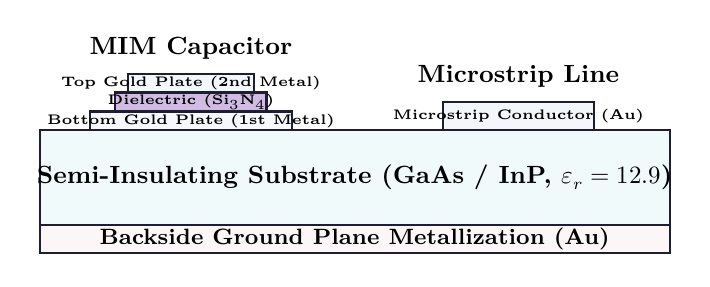
\begin{tikzpicture}[x=1.6cm, y=1.2cm]
  % Substrate
  \draw[line, fill=hdrteal!40] (0,0) rectangle (5.0,1.0);
  \node at (2.5,0.5) {\small\textbf{Semi-Insulating Substrate (GaAs / InP, $\varepsilon_r = 12.9$)}};
  
  % Ground Plane
  \draw[line, fill=hdrred!40] (0,-0.3) rectangle (5.0,0);
  \node at (2.5,-0.15) {\footnotesize\textbf{Backside Ground Plane Metallization (Au)}};
  
  % MIM Capacitor - Bottom Plate
  \draw[line, fill=hdrblue!50] (0.4,1) rectangle (2.0,1.2);
  \node at (1.2,1.1) {\tiny\textbf{Bottom Gold Plate (1st Metal)}};
  
  % MIM Dielectric
  \draw[line, fill=mypurple!30] (0.6,1.2) rectangle (1.8,1.4);
  \node at (1.2,1.3) {\tiny\textbf{Dielectric ($\text{Si}_3\text{N}_4$)}};
  
  % MIM Top Plate
  \draw[line, fill=hdrblue!60] (0.7,1.4) rectangle (1.7,1.6);
  \node at (1.2,1.5) {\tiny\textbf{Top Gold Plate (2nd Metal)}};
  
  % Microstrip Line
  \draw[line, fill=hdrblue!60] (3.2,1) rectangle (4.4,1.3);
  \node at (3.8,1.15) {\tiny\textbf{Microstrip Conductor (Au)}};
  
  % Labels
  \node[anchor=south] at (1.2,1.65) {\small\textbf{MIM Capacitor}};
  \node[anchor=south] at (3.8,1.35) {\small\textbf{Microstrip Line}};
\end{tikzpicture}
\end{tcolorbox}

\begin{tcolorbox}[examplebox, title={MIM Capacitor Calculation}]
  \textbf{Problem:} Calculate the required area of a Silicon Nitride ($\text{Si}_3\text{N}_4$, $\varepsilon_r = 7.5$) MIM capacitor to achieve a capacitance of $C = 10\text{ pF}$ if the dielectric thickness is $d = 2000\text{ \AA}$ ($200\text{ nm}$).
  \tcblower
  \textbf{Solution:}
  Using the parallel-plate capacitance formula:
  \begin{equation}
    C = \frac{\varepsilon_0 \varepsilon_r A}{d} \implies A = \frac{C \cdot d}{\varepsilon_0 \varepsilon_r}
  \end{equation}
  Given: $C = 10 \times 10^{-12}\text{ F}$, $d = 200 \times 10^{-9}\text{ m}$, $\varepsilon_0 = 8.854 \times 10^{-12}\text{ F/m}$, $\varepsilon_r = 7.5$.
  \begin{equation}
    \begin{aligned}
      A &= \frac{(10 \times 10^{-12}) \times (200 \times 10^{-9})}{(8.854 \times 10^{-12}) \times 7.5} \\
      &= \frac{2 \times 10^{-18}}{6.6405 \times 10^{-11}} = 3.0118 \times 10^{-8}\text{ m}^2 = 0.0301\text{ mm}^2
    \end{aligned}
  \end{equation}
  For a square capacitor plate of length $L$:
  \begin{equation}
    L = \sqrt{A} = \sqrt{0.0301\text{ mm}^2} \approx 0.1735\text{ mm} = 173.5\text{ }\mu\text{m}
  \end{equation}
\end{tcolorbox}

% ===============================================================================
% 3. ENCAPSULATION AND MOUNTING OF ACTIVE DEVICES
% ===============================================================================
\section{Encapsulation and Mounting of Active Devices}

\subsection{Active Device Mounting Techniques}
In Hybrid MICs, discrete active semiconductor chips (diodes, MESFETs, HBTs) must be attached to the substrate and interconnected to microstrip lines. Three primary mounting techniques are utilized:

\begin{enumerate}[leftmargin=*, itemsep=5pt]
  \item \textbf{Wire Bonding (Thermosonic / Ultrasonic):}
    \begin{itemize}[leftmargin=*, noitemsep]
      \item Fine Gold ($\text{Au}$) wires ($17.5 - 25\text{ }\mu\text{m}$ diameter) connect die pads to substrate traces.
      \item \textit{Drawback:} Introduces parasitic series inductance $L_s \approx 1\text{ nH/mm}$. At $20\text{ GHz}$, a $1\text{ mm}$ wire bond introduces an inductive reactance $X_L = 2\pi f L_s = 2\pi (20 \times 10^9) (10^{-9}) = 125.66\text{ }\Omega$, destroying impedance matching!
    \end{itemize}
  \item \textbf{Flip-Chip Bonding:}
    \begin{itemize}[leftmargin=*, noitemsep]
      \item The semiconductor die is inverted face-down and attached directly to substrate pads via solder bumps or gold pillars ($20 - 50\text{ }\mu\text{m}$ height).
      \item Reduces parasitic series inductance by over $95\%$ ($L_s < 0.05\text{ nH}$), enabling performance up to $100\text{ GHz}$.
    \end{itemize}
  \item \textbf{Tape Automated Bonding (TAB):}
    \begin{itemize}[leftmargin=*, noitemsep]
      \item Patterned copper foil leads on a flexible polyimide film are gang-bonded simultaneously to die pads.
    \end{itemize}
\end{enumerate}

\subsection{Encapsulation and Package Requirements}
Packaging protects delicate GaAs/InP devices from environmental humidity, oxidation, and mechanical stress while providing a low-reflection $50\text{ }\Omega$ RF path.

\begin{tcolorbox}[defbox, title={Hermetic Packaging}]
  \textbf{Hermetic Packaging} encloses MIC/MMIC circuits inside glass-sealed ceramic or laser-welded metal housings filled with dry nitrogen, preventing moisture ingress and long-term performance degradation.
\end{tcolorbox}

% ===============================================================================
% QUICK REVISION PAGE
% ===============================================================================
\newpage
\begin{center}
  {\large\bfseries\color{myred} Quick Revision --- Module 1}\\[3pt]
  {\small\color{mydark} Introduction to MIC \& MMIC $|$ OE-EC804B}
\end{center}
\noindent{\color{myred}\rule{\linewidth}{1.2pt}}
\vspace{4pt}

\begin{tcolorbox}[formulabox, title={\textbf{Key Concepts and Metrics at a Glance}}]
\renewcommand{\arraystretch}{1.35}
\begin{tabularx}{\linewidth}{>{\raggedright\arraybackslash\bfseries}p{4.5cm} X}
Hybrid MIC (HMIC) & Passives on dielectric substrate ($\text{Al}_2\text{O}_3$); discrete active dies wire-bonded. \\[4pt]
Monolithic MIC (MMIC) & Passives, active devices, and lines fabricated monolithically on single GaAs/InP wafer. \\[4pt]
Substrate Materials & GaAs ($\varepsilon_r=12.9, \mu_e=8500$), InP ($\varepsilon_r=12.4$), GaN ($\varepsilon_r=8.9, 3\text{ MV/cm}$). \\[4pt]
MIM Capacitance & $C = \frac{\varepsilon_0 \varepsilon_r A}{d}$ \quad ($\text{Si}_3\text{N}_4$ dielectric, $\varepsilon_r = 7.5$). \\[4pt]
Wire Bond Parasitic & $L_s \approx 1\text{ nH/mm} \implies X_L = 2\pi f L_s$; mitigated by Flip-Chip bonding ($<0.05\text{ nH}$). \\
\end{tabularx}
\end{tcolorbox}

\begin{tcolorbox}[defbox, title={\textbf{One-Line Definitions}}]
  \begin{itemize}[leftmargin=*, noitemsep]
    \item \textbf{MMIC:} An integrated circuit containing all active and passive microwave components on a single semiconductor chip.
    \item \textbf{MIM Capacitor:} Metal-Insulator-Metal thin film capacitor providing high capacitance density in MMICs.
    \item \textbf{Loss Tangent ($\tan\delta$):} Ratio of imaginary to real permittivity ($\varepsilon''/\varepsilon'$) measuring dielectric RF dissipation.
    \item \textbf{Flip-Chip Bonding:} Surface-mount method bonding an inverted chip face-down via solder bumps, eliminating wire bond inductance.
  \end{itemize}
\end{tcolorbox}

\begin{tcolorbox}[exambox, title={\textbf{Frequently Asked / Viva Questions}}]
  \begin{enumerate}[topsep=0pt, label=\textbf{Q\arabic*.}, itemsep=5pt]
    \item \Q{Compare Hybrid MICs and Monolithic MICs.}
    HMICs use separate dielectric substrates with individually mounted active chips. MMICs fabricate all active and passive components simultaneously on a single semiconductor substrate (GaAs/InP).

    \item \Q{Why is GaAs preferred over Silicon for MMICs?}
    GaAs is a direct bandgap semiconductor with semi-insulating resistivity ($\rho > 10^7\text{ }\Omega\cdot\text{cm}$) and higher electron mobility ($\mu_e \approx 8500\text{ cm}^2/\text{V}\cdot\text{s}$ vs $1400$ for Si), providing low RF substrate losses.

    \item \Q{What are the advantages of MMICs over discrete microwave circuits?}
    Small size, low weight, high reliability, high reproducibility, elimination of wire bond parasitics, and low mass-production cost.

    \item \Q{Explain Thin Film technology in MIC fabrication.}
    Thin film technology deposits metal and dielectric films ($<5\text{ }\mu\text{m}$) via sputtering or evaporation, using photolithography to achieve high-precision line widths down to sub-micron scales.

    \item \Q{What materials are used for thin film resistors and capacitors?}
    Resistors use Tantalum Nitride ($\text{TaN}$) or Nickel Chromium ($\text{NiCr}$). Capacitors use Metal-Insulator-Metal (MIM) with $\text{Si}_3\text{N}_4$ or $\text{SiO}_2$ dielectrics.

    \item \Q{What is the main electrical drawback of wire bonding at microwave frequencies?}
    Wire bonds introduce parasitic series inductance ($L_s \approx 1\text{ nH/mm}$), causing significant impedance mismatches above $12\text{ GHz}$.

    \item \Q{How does Flip-Chip bonding overcome wire bond parasitics?}
    Flip-Chip bonding mounts the chip face-down directly onto substrate pads using short solder bumps, reducing parasitic inductance by over $90\%$.

    \item \Q{Why is high thermal conductivity critical for MMIC substrate materials?}
    High-power active devices generate significant heat in a small area; high thermal conductivity prevents thermal breakdown and maintains transistor gain.

    \item \Q{Define loss tangent ($\tan\delta$) and its significance in MICs.}
    Loss tangent $\tan\delta = \epsilon'' / \epsilon'$ quantifies dielectric power loss; lower $\tan\delta$ minimizes attenuation in planar transmission lines.

    \item \Q{What is Hermetic Sealing and why is it necessary for MMICs?}
    Hermetic sealing provides an airtight ceramic/metal package protecting unpassivated GaAs active devices from moisture and atmospheric degradation.
  \end{enumerate}
\end{tcolorbox}

\end{document}
